\section{Optimization}
\label{sect:optimization}

In the fourth and last phase of the pipeline, we improve on the initial drawing of the boundary graph while preserving its combinatorial embedding of the map. We move the vertices around to optimize statistical accuracy and other quality metrics that we are interested in. We can also subdivide edges to create more degrees of freedom or get rid of subdivision vertices (vertices with degree 2) when we don't need those degrees of freedoms any more.

\begin{figure}[H]
	\centering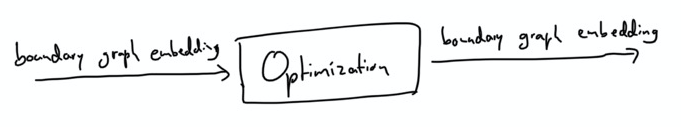
\includegraphics[width=0.9\textwidth]{Resources/Pipeline-Optimization.png}
	\caption{Input and output of the optimization phase.}
	\label{fig:pipeline-optimization}
\end{figure}
